%
%  This simple example illustrates how documents can be
%  split into smaller segments, each segment processed
%  by latex2html separately.  This document can be
%  processed through latex and latex2html with the
%  corresponding makefile.
%

\documentclass{article}         % Must use LaTeX 2e
\usepackage[plainpages=false, colorlinks=true, citecolor=black, filecolor=black, linkcolor=black, urlcolor=black]{hyperref}		
\usepackage[left=.75in,right=.75in,top=.75in,bottom=.75in]{geometry}
\usepackage{makeidx,color,boxedminipage}
\usepackage{graphicx,float}
\usepackage{amsmath,amsthm,amsfonts,amscd,amssymb} 

%%%%%%%%%%%%%%%%%%%%%%%%%%%%%%%%%%%%%%%%%%%%%%%%%%%%%%%%%%%%%%%%%%%%%%
%	Some math support.					     %
%%%%%%%%%%%%%%%%%%%%%%%%%%%%%%%%%%%%%%%%%%%%%%%%%%%%%%%%%%%%%%%%%%%%%%
%
%	Theorem environments (these need the amsthm package)
%
%% \theoremstyle{plain} %% This is the default

\newtheorem{thm}{Theorem}[section]
\newtheorem{cor}[thm]{Corollary}
\newtheorem{lem}[thm]{Lemma}
\newtheorem{prop}[thm]{Proposition}
\newtheorem{ax}{Axiom}

\theoremstyle{definition}
\newtheorem{defn}{Definition}[section]

\theoremstyle{remark}
\newtheorem{rem}{Remark}[section]
\newtheorem*{notation}{Notation}
\newtheorem*{exrcs}{Exercise}
\newtheorem*{exmple}{Example}

%\numberwithin{equation}{section}


%%%%%%%%%%%%%%%%%%%%%%%%%%%%%%%%%%%%%%%%%%%%%%%%%%%%%%%%%%%%%%%%%%%%%%
%	Macros.							     %
%%%%%%%%%%%%%%%%%%%%%%%%%%%%%%%%%%%%%%%%%%%%%%%%%%%%%%%%%%%%%%%%%%%%%%
%
%	Here some macros that are needed in this document:

\newcommand{\motion}{\mathbf{\varphi}}
\newcommand{\hmotion}{\mbox{\boldmath $\hat{\varphi}$}}
\newcommand{\cauchy}{\mbox{\boldmath $\sigma$}}
\newcommand{\eqn}[1]{(\ref{#1})}
\newcommand{\hOmega}{\hat{\Omega}}
\newcommand{\homega}{\hat{\omega}}
\newcommand{\nphalf}{n+\frac{1}{2}}
\newcommand{\nmhalf}{n-\frac{1}{2}}
\newcommand{\kmhalf}{k-\frac{1}{2}}
\newcommand{\kphalf}{k+\frac{1}{2}}
\newcommand{\picdir}{pdffig/}

\newcommand{\re}{\mathbb R}
\newcommand{\Ex}[2]{\mathcal{E}^{#2}[#1]}
%\newcommand{\log}{\text{log}[#1]}
\newcommand{\Tr}{\mathbf{Tr}}
\newcommand{\etal}{\textit{et al. }}

\newcommand{\eq}[1]{Eq.~(\ref{#1})}
\newcommand{\Fig}[1]{Fig.~\ref{#1}}

\renewcommand{\v}[1]{\ensuremath{\mathbf{#1}}}
\newcommand{\vo}[1]{\ensuremath{\boldsymbol{#1}}}
\newcommand{\pderiv}[2]{\frac{\partial #1}{\partial #2}}

\newcommand{\eps}{\boldsymbol{\epsilon}}
\newcommand{\Nu}{\boldsymbol{\nu}}
\newcommand{\Ps}{\boldsymbol{\Psi}}
\newcommand{\xii}{\boldsymbol{\xi}}
\newcommand{\Al}{\boldsymbol{\alpha}}
\newcommand{\x}{\mathbf{x}}
\newcommand{\s}{\mathbf{s}}
\newcommand{\C}{\mathbf{C}}
\newcommand{\uu}{\mathbf{u}}
\newcommand{\z}{\mathbf{z}}
\newcommand{\q}{\mathbf{q}}
\newcommand{\A}{\mathbf{A}}
\newcommand{\B}{\mathbf{B}}
\newcommand{\K}{\mathbf{K}}
\newcommand{\f}{\mathbf{f}}
\newcommand{\hc}{\mathbf{H}}
\newcommand{\R}{\mathbf{R}}
\newcommand{\G}{\mathbf{G}}
\newcommand{\y}{\mathbf{y}}
\newcommand{\Y}{\mathbf{Y}}
\newcommand{\teta}{\boldsymbol{\theta}}
\newcommand{\Teta}{\boldsymbol{\Theta}}
\newcommand{\pe}{\hat{\mathbf{p}}}
\newcommand{\pl}{\mathbf{p}^{(l)}}
\newcommand{\pt}{\mathbf{p}^\text{true}}

\newcommand{\kk}{\mathcal{K}}
\newcommand{\p}{\mathcal{P}}
%\DeclareMathOperator{\Exp}{E}
\newcommand{\V}{{\mathpzc{V}}}
\newcommand{\E}{{\mathpzc{E}}}

\newcommand{\bs}{b}
\newcommand{\bv}{\mathbf{b}}
\newcommand{\bme}{z}
\newcommand{\bvm}{\tilde{\bv}}
\newcommand{\xg}{x^G}
\newcommand{\yg}{y^G}
\newcommand{\kbf}{\mathbf{k}}
\newcommand{\mbf}{\mathbf{m}}
\newcommand{\Pbf}{\mathbf{P}}
\newcommand{\Rbf}{\mathbf{R}}
\newcommand{\Vbf}{\mathbf{V}}
\newcommand{\xbf}{\mathbf{x}}
\newcommand{\Xbf}{\mathbf{X}}
\newcommand{\Ybf}{\mathbf{Y}}
\newcommand{\zbf}{\mathbf{z}}
\newcommand{\Zbf}{\mathbf{Z}}
\newcommand{\mubf}{\boldsymbol{\mu}}
\newcommand{\nubf}{\boldsymbol{\nu}}
\newcommand{\im}{\mathrm{i}}
\newcommand{\Gammabf}{\mathbf{\Gamma}}
\newcommand{\Cbf}{\mathbf{C}}
\newcommand{\Sigmabf}{\boldsymbol{\Sigma}}
\newcommand{\zcond}{\mathbf{z}\mid\mu}
\newcommand{\zcondbf}{\mathbf{z}\mid\boldsymbol{\mu}}
\newcommand{\signalG}{\mathcal{G}\paren{\mu,\mathbf{k}}}
\newcommand{\Gscript}{\mathcal{G}}
\newcommand{\sumnn}{\sum\limits_{n=1}^N}

\newcommand{\arr}[2]{\begin{array}{#1} #2 \end{array}}
\newcommand{\lbrcarray}[2]{\left\{\arr{#1}{#2}\right.}
\newcommand{\rbrcarray}[2]{\left.\arr{#1}{#2}\right\}}
\newcommand{\argminx}{\arg\min_X}
\newcommand{\Nscript}{\mathcal{N}}

%\DeclareMathOperator{\diag}{diag} 
\newcommand{\brkarray}[2]{\bracket{\arr{#1}{#2}}}

\title{WIP - Synthetic MR }
\author{}
\begin{document}                % The start of the document
%%%%%%%%%%%%%%%%%%%%%%%%%%%%%%%%%%%%%%%%%%%%%%%%%%%%%%%%%%%%%%%%
\section{WIP - Model Data Fusion}\label{da}
%%%%%%%%%%%%%%%%%%%%%%%%%%%%%%%%%%%%%%%%%%%%%%%%%%%%%%%%%%%%%%%%
After finding the optimal values of the control parameter $\kk$, we can proceed and perform the model-data fusion to get a better understanding about the uncertainties involved in parameters $\p$.
The fusion of observational data with mathematical model predictions promises to provide greater understanding of physical phenomenon than either approach alone can achieve. In here, a minimum variance framework is being used for model - data fusion. Based on minimum variance technique, posterior statistics of parameter $\p$ can be written as:

\begin{eqnarray}
\hat{\p}^+=\hat{\p}^-+\K[z-\underbrace{\Ex{h(\kk,\p)}{-}}_{h^-}]\label{minvarmean}\\
\Sigma^+=\Sigma^-+\K\Sigma_{hh}\K^T\label{minvarvar}
\end{eqnarray}
where, %$z\equiv \tilde{M}_{TD}$ and 
the gain matrix $K$ is given by
\begin{eqnarray}\label{kgain}
\K=\Sigma_{\p z}\left(\Sigma_{hh}^-+\R\right)^{-1}
\end{eqnarray}

Here, $\hat{\p}^-$ and $\hat{p}^+$ represent prior and posterior values of the mean for parameter vector $\p$, respectively:
\begin{eqnarray}
\hat{\p}^-\equiv \Ex{\p}{-}=\int \p^- p(\p)d\p \label{Pprior}
\hat{\p}^+\equiv \Ex{\p}{+}=\int \p^+ p(\p)d\p \label{Pposterior}
\end{eqnarray}
where, $p(\p)$ denotes the probability density function of parameter $\p$. Similarly, the prior and posterior covariance matrices $\Sigma^{-}$ and $\sigma^+$ can be written as:

\begin{eqnarray}
\Sigma^-\equiv\Ex{(\p-\hat{\p}^-)(\p-\hat{\p}^-)^T}{}\\
\Sigma^+\equiv\Ex{(\p-\hat{\p}^+)(\p-\hat{\p}^+)^T}{}
\end{eqnarray}

The matrices $\Sigma_{\p z}$ amd $\Sigma_{hh}$ are defined as:

\begin{eqnarray}
\Sigma_{\p z} \equiv\Ex{(\p-\hat{\p})(h-\hat{h}^-)^T}{}\\
\Sigma_{hh} \equiv\Ex{(h-\hat{h}^-)(h-\hat{h}^-)^T}{}
\end{eqnarray}

\eq{minvarmean} along with \eq{minvarvar} provide posterior mean and covariance of parameter $\p$ given observation data $\tilde{z}$ and model predictions $h(\kk,\p)$.
We emphasize here that the optimal values of $\kk$, obtained from \eq{mimax}, are used in \eq{minvarmean}.

%%%%%%%%%%%%%%%%%%%%%%%%%%%%%%%%%%%%%%%%%%%%%%%%%%%%%%%%%%%%%%%%
\section{MI Approximations: Maximizing the Variance}
%%%%%%%%%%%%%%%%%%%%%%%%%%%%%%%%%%%%%%%%%%%%%%%%%%%%%%%%%%%%%%%%


Unfortunately, evaluation of mutual information and solving the above
optimization problem is computationally intractable for most of the practical
applications. Hence, one needs to simplify the original optimization problem
and find the approximate solution for optimal location of each observation. A
simpler alternative in finding useful $k-$space locations is to maximize the
entropy (uncertainty) in model outputs $\mathcal{U}$, instead of maximizing the
mutual information $I(\mu;z)$ \cite{krause2008}. Based on information theory,
the entropy of $\mathcal{U}$, denoted by $h(\mathcal{U})$ is defined as:
%

\begin{equation}\label{entropy}
h(\mathcal{U})=-\int_{\mathcal{U}} ln\left(p(\mathcal{U})\right)p(\mathcal{U})d\mathcal{U}
\end{equation}
where, $p(\mathcal{U})$ is the probability density function of $\mathcal{U}$. % As well, $h(\mathcal{U}|z)$ represents the entropy of $\mathcal{U}$, given the measurement $z$.
One can simplify the problem by just maximizing the entropy of model outputs,
instead of maximizing the mutual information. We emphasize here that this
simplification may have its drawback in not giving the \textit{globally}
optimal locations on $k-$space, but as we will show in the following, it will
result in great simplification of the problem. 

To proceed with maximizing the entropy $h(\mathcal{U})$, we first note that
based on Maximum Entropy Principle \cite{cover2012elements}, probability
density function $p(\mathcal{U})$ can be parametrized in terms of its central
moments as

\begin{equation}\label{pu_entropy}
p(\mathcal{U})=\lim_{N\rightarrow \infty} \left(e^{\sum\limits_{n=0}^N \lambda_n (\mathcal{U}-\hat{\mathcal{U}})^n}\right),\quad \lambda_n \in \re
\end{equation}

where, $\hat{\mathcal{U}}$ is provided by \eqref{expx1U}. By substituting
\eq{pu_entropy} in \eq{entropy}, we will have: $  $
\begin{align}
h(\mathcal{U})=-\int_{\mathcal{U}} \lim_{N\rightarrow \infty} \left(\sum\limits_{n=0}^\infty \lambda_n (\mathcal{U}-\hat{\mathcal{U}})^n\right) p(\mathcal{U})d(\mathcal{U})\nonumber\\
= \lim_{N \rightarrow \infty} (-\lambda_0 - \sum\limits_{n=2}^{N} \lambda_n m_n) \label{entropy_moments}
\end{align}
where, $m_n$s are the central moments of $\mathcal{U}$, defined by \eq{expx1_ctrU}. Hence, entropy of $p(\mathcal{U})$ can be described in terms of its central moments, as shown in \eq{entropy_moments}. Now, by approximating $p(\mathcal{U})$ with its first two moments and truncating the above expansion (i.e. letting $N=2$), we have 

\begin{equation}\label{entropy_var}
h(\mathcal{U})\simeq -\lambda_0-\lambda_2 m_2,\quad \lambda_0,\lambda_2 \in \re
\end{equation}
Therefore, to maximize the entropy one can only maximize the variance, i.e.
\begin{eqnarray}\label{entropy_var_max}
\max_{K} h(\mathcal{U})= -\lambda_0 -\lambda_2 \max_{K}(m_2), \quad \lambda_0,\lambda_2 \in \re
\end{eqnarray}
\textcolor{black}{subject to:
\begin{equation}\label{sparsity_con}
|K^i-K^j|\geq N_d,\quad \forall\ i,j\in 1,2,\cdots,N,\quad i\neq j 
\end{equation}}
where, $|K^i-K^j|=|(k_x^i,k_y^i,k_z^i)-(k_x^j,k_y^j,k_z^j)|$ denotes the
distance between the $i^{th}$ and $j^{th}$ locations on $k-$space and
$m_2=Var(\mathcal{U})$ is defined from \eq{expx1_ctrU}. Hence, the locations on
$k-$space with the highest value of variance for $\mathcal{U}$ are a good
approximation of optimal locations for data observations. 

\textcolor{black}{\eq{sparsity_con} is considered to ensure that every distinct
pair of $k-$space observations are at least by a distance $N_d$ apart from each
other. This constraint is used in order to compensate possible dependencies
that can be introduced due to approximation of the original problem. We assumed
$N_d=1$ through this manuscript.}

\textcolor{black}{One should note that different order of truncation (i.e.
different values of $N$) can be used to approximate the entropy in
\eq{entropy_moments}. Clearly, higher order approximation (greater values of
$N$) leads to more accurate approximation of entropy. However, the downside of
using higher order terms is that one needs to find the corresponding
$\lambda_n$ coefficients for each term. Finding corresponding $\lambda_n$
coefficients requires solving an optimization problem which could increase
computational cost of the whole procedure. Hence, lower order approximation of
entropy is of more interest due to real time applications of the proposed
technique.}

%As explained in section \ref{subsec:kspace}, solution of associated optimization problem with maximizing mutual information can be computationally intractable in presence of large number of measurements. In addition, evaluation of mutual information $I(\mu;z)$ can be computationally expensive due to associated integrations in \eq{mutual_info}. A simpler alternative to avoid these complexities is to find the locations on $k-$space which posses the highest variability in model predictions. To achieve this, one first needs to perform non-uniform Fourier transform on the Pennes bioheat model outputs using \eq{ymodel} and then, variance of model predictions can be  calculated as given in \eq{expx1_ctrU}, i.e.
%
%\begin{equation}\label{varkspace}
%Var(\mathcal{U})=\sum_{q=1}^{M} w_q(\mathcal{U}(\x,\mu(\xii^q),t)-\hat{\mathcal{U}})^2
%\end{equation}
%where, $\hat{\mathcal{U}}$ is the expected value of $\mathcal{U}$, calculated using \eq{expx1U}. Now, the locations on $k-$space with highest value of the variance are the \textit{most useful} locations for data observations. 
The intuition behind the idea of maximizing the variance is that the points on
$k-$space with lower value of variance are less sensitive to model
perturbations (resulted from parameter uncertainties) and vice versa. Hence, it
is better to select the points on $k-$space with highest sensitivity with
respect to model uncertainties. For instance, a point with zero variance on
$k-$space will not be a good candidate for data observation since no matter
what the values of uncertain parameters are, model output will always be the
same at that specific point. On the other hand, a point on $k-$space with large
value of variance means that the model output at that location is
\textit{highly sensitive} to model uncertainties. Hence, a measurement at that
$k-$space location would be of more interest. Therefore, the points with
highest values of variance of $\mathcal{U}$ are \textit{better candidates} for
data observations. 

%Note that against the mutual information, calcuation of variance of model outputs is very simple and computationally affordable. In addition, solving the optimization problem associated with finding the points with highest values of variance is a much simpler task, comparing with solution of \eq{cost3}.


{\color{red}(@dmitchell412 need Variance calculation algorithm compiled here with Quadrature)}

 
%%%%%%%%%%%%%%%%%%%%%%%%%%%%%%%%%%%%%%%%%%%%%%%%%%%%%%%%%%%%%%%%
\section{WIP - Echo train length }\label{ModelFidelity}
%%%%%%%%%%%%%%%%%%%%%%%%%%%%%%%%%%%%%%%%%%%%%%%%%%%%%%%%%%%%%%%%


% http://mriquestions.com/fse-parameters.html
% http://mriquestions.com/what-is-fsetse.html

In conventional spin-echo imaging, two basic timing parameters are
required, repetition time (TR) and echo time (TE), Figure~\ref{fig:echotrain}(a).
Similar to
fast spin echo (FSE) imaging, 
the acquistion is setup to acquire multiple lines of k-space in a single TR.
In this situation,
TE is replaced by effective echo
time  and addition parameters are needed: 

\begin{itemize}
\item TE$_\text{eff} \equiv$ the time at which the central lines of k-space are being filled.
\item Number of echoes $\equiv$ called echo train length (ETL)
\item Time between echoes $\equiv$ called echo spacing (ESP) 
\end{itemize}



\begin{figure}[h] 
\begin{tabular}{ccc}
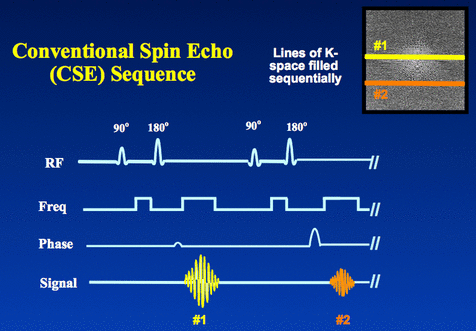
\includegraphics[width=.3\textwidth]{\picdir/7162303.png}
&
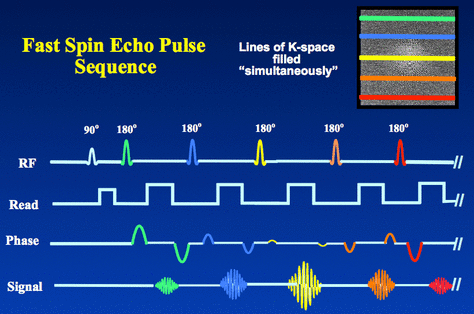
\includegraphics[width=.3\textwidth]{\picdir/5013564.png}
&
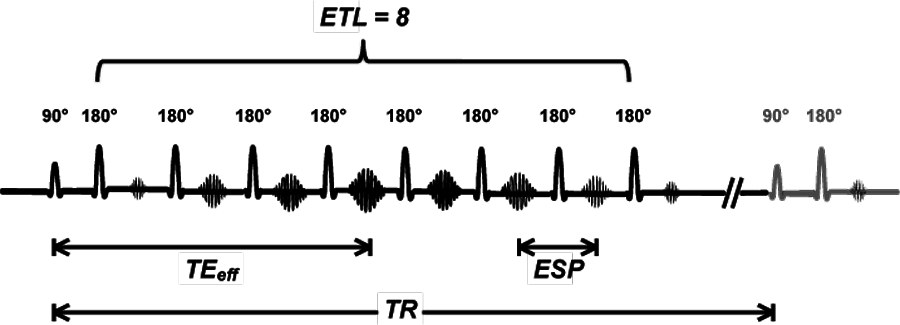
\includegraphics[width=.3\textwidth]{\picdir/3316708_orig.png}
\\
(a) & (b) & (c) \\
\end{tabular}
\caption{ 
(a)
}\label{fig:echotrain}
\end{figure}


{\color{red}
   TODO - do we need to update signal model for multiple read out lines ? 
}

%%%%%%%%%%%%%%%%%%%%%%%%%%%%%%%%%%%%%%%%%%%%%%%%%%%%%%%%%%%%%%%%
\section{WIP - k-space signal model}
%%%%%%%%%%%%%%%%%%%%%%%%%%%%%%%%%%%%%%%%%%%%%%%%%%%%%%%%%%%%%%%%


{\color{red} @wstefan @kenphwang need to develop full k-space model of echo train trajectories for subsampling.}

Consider the schematic of the pulse sequence for the  acquistion provided in
Figure~\ref{fig:Pulsesequencemfgre}(a).
For a  given tissue, $\Omega \subset \mathbb{R}^3$,
with heterogenious intrinistic relaxation properties $T1(r)$ and $T2^*(r)$
we will assume a multi-echo signal, $s_l(t,n)\in\mathbb{C}$ ,
from the l-th coil at the n-th echo 
of the form of a linear combination of damped exponentials. 
The signal strength is dependent on the coil sensitivity $c_l(r)$.
\begin{equation}
\label{multiechosignalmodel}
\begin{split}
 s_l(t,n) = \int_\Omega c_l(r)  w[n] e^{-i \int_0^t \gamma \vec{G}(\tau)\cdot r d \tau} \; dr
\qquad
 w[n]  = \sum_j^{N_\text{species}} 
 C_j \Lambda_j^n 
  \qquad  \qquad n = 0,1,2,\dots,N_\text{echo}-1
\\
\Lambda_j^n  = e^{-\left( 
\underbrace{i\; \Delta B_{0_j}(r) }_\text{off-resonance} 
+
\frac{1}{T2^*_j} \right) \left( \text{TE} + n \; \text{ESP}\right) } 
\quad  \quad
C_j = \frac{M_{0_j} \sin \left(\gamma \theta_N \right)\left( 1- e^{-TR/T1_j}\right)}{\left( 1- \cos \left(\gamma \theta_N \right) e^{-TR/T1_j}\right)}
e^{-i  \phi_j} 
\in  \mathbb{C} 
\end{split}
\end{equation}

Each weighted exponential, $C_j \Lambda_j$, represents a distinct chemical species,
ie water, fat, sodium hydroxide, etc. 
The complex amplitude,
$C_j \in \mathbb{C}$, 
depends on (1) acquisition parameters - repetition time, TR,
and flip angle, $\theta_N$, as well as (2) tissue dependent properties -
 spin lattice relaxation,  $T1_j$,
 proton density $M_{0_j}$, and
 initial phase offset, $\phi_j$.
Similarly, the complex exponential, $\Lambda_j$,
depends on (1) acquisition parameters - echo time, TE,
echo spacing , ESP, as well as (2) tissue dependent properties -
 spin spin relaxation,  $T2^*_j$, and tissue depending off-resonsance
arising from temperature change, motion, and/or susceptibility, 
$\Delta B_{0_j}(r)$.
\[
 \Delta B_{0_j}(r) = 
\left\{ 
\begin{split}
                2\pi f_j = 2\pi \underbrace{\alpha B_0 \Delta T_j(r)}_{f_j} & \qquad \text{temperature}   
\\
                ... =      & \qquad \text{susceptibility}   
\\
                ... =      & \qquad \text{motion}   
\end{split}
\right.
\]

%%%%%%%%%%%%%%%%%%%%%%%%%%%%%%%%%%%%%%%%%%%%%%%%%%%%%%%%%%%%%%%%
\section{MI Calculations}
%%%%%%%%%%%%%%%%%%%%%%%%%%%%%%%%%%%%%%%%%%%%%%%%%%%%%%%%%%%%%%%%



A more direct calculation of the entropy is given as
\[
   p(z) = \int_\theta p(z|\theta) p (\theta) d \theta = \sum_q \omega_q p(z|\theta_q)
\]
\[ \begin{split}
 MI = H(z) &  = \int_z p(z) ln \; p(z) \; dz 
          = \int_z ln \; p(z) \; \int_\theta p(z|\theta) p (\theta) d \theta   \; dz  
    \approx \int_z ln \; p(z)  \sum_q \omega_q p(z|\theta_q)  \; dz 
      \\ &  
          =  \sum_q \omega_q \int_z ln \; p(z)  p(z|\theta_q)  \; dz 
      \underbrace{ \approx }_{?}\sum_q \omega_q \sum_r \omega_{r} ln \; p(x_r + g(\theta_q) )
      \underbrace{ \approx }_{?}\sum_q \omega_q \sum_r \omega_{r} ln \left( \sum_l \omega_l p( x_r + g(\theta_q) |\theta_l) \right) 
      \\ &  
      \underbrace{ \propto }_{?}\sum_q \omega_q \sum_r \omega_{r} ln \left( \sum_l \omega_l e^\frac{ x_r + g(\theta_q) - g(\theta_l)}{\sigma} \right) 
\end{split}
\]

Derivatives for optimization with respect to control parameters $\kappa_i$ are computed with chain rule and sensitivities:
\[
\frac{\partial \; MI}{\partial \kappa_i} = 
      \sum_q \omega_q \sum_r \omega_{r} ln \left( \sum_l \omega_l e^\frac{ x_r + g(\theta_q) - g(\theta_l)}{\sigma} 
       \left( \frac{\partial g(\theta_q)}{\partial u}\frac{\partial u}{\partial \kappa_i} 
           -  \frac{\partial g(\theta_l)}{\partial u}\frac{\partial u}{\partial \kappa_i} 
      \right) \right) 
\]

%\begin{figure}[h] 
%\centering
%\begin{tabular}{ccc}
%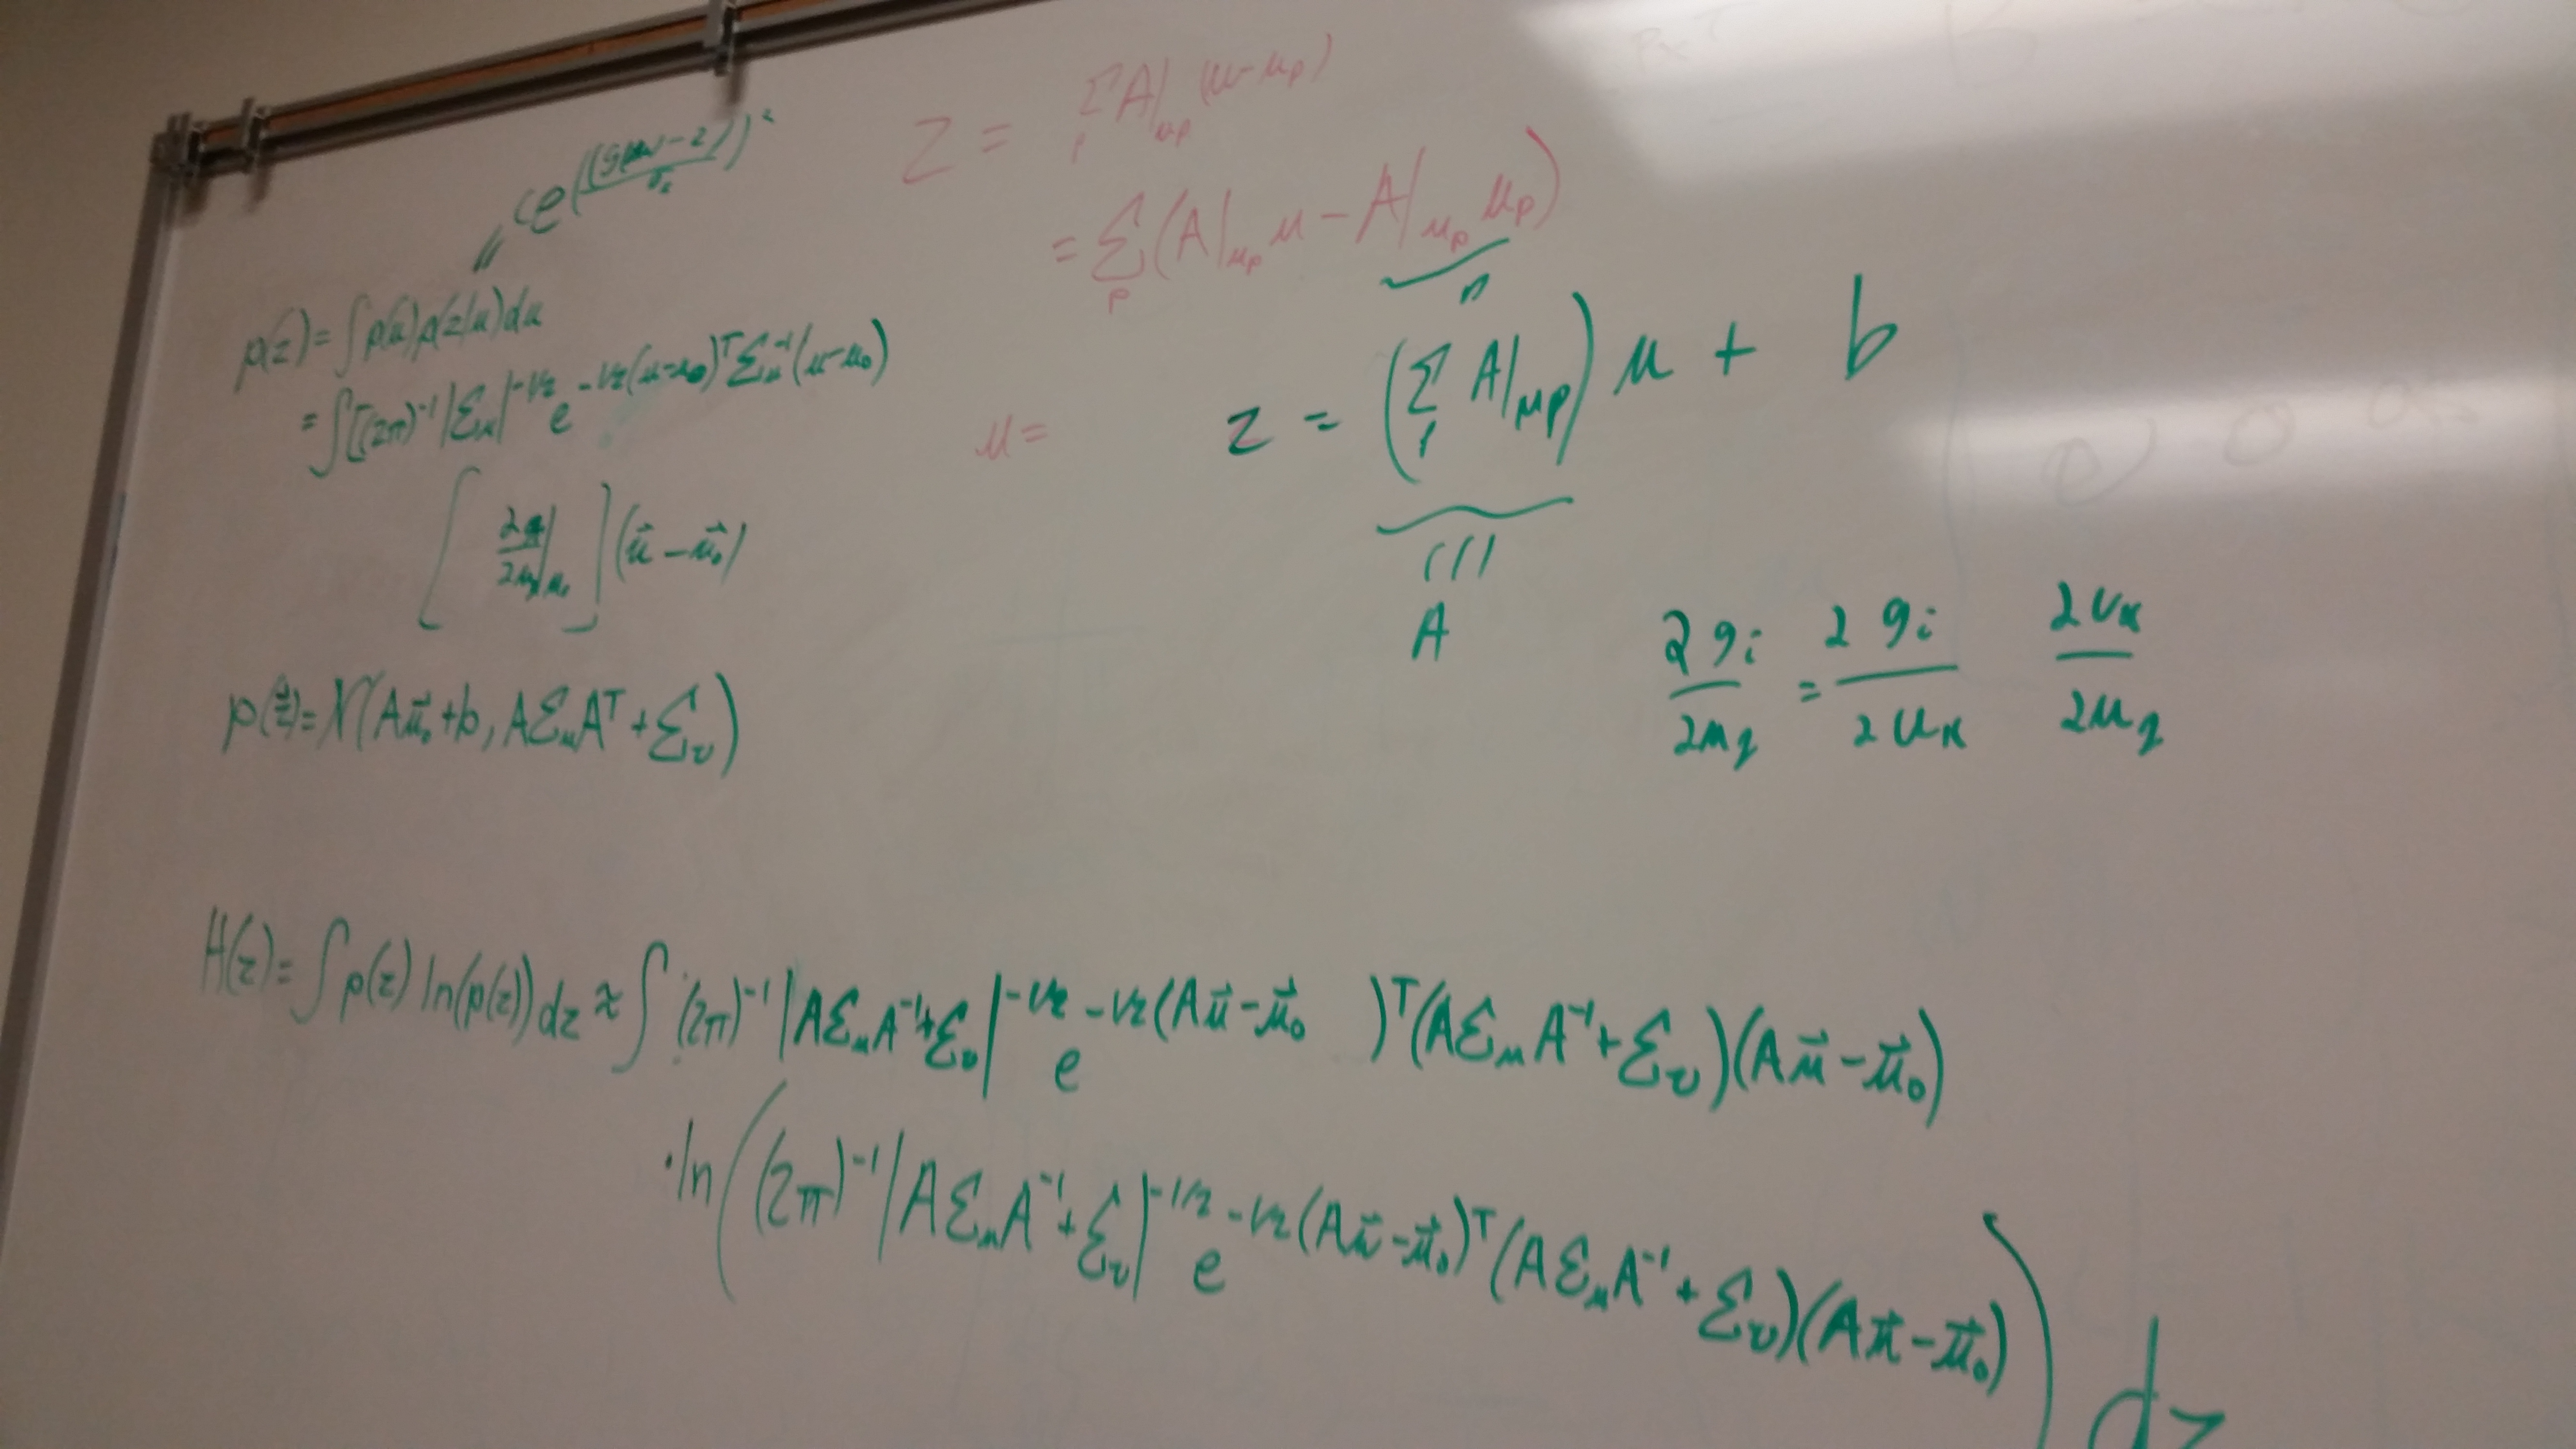
\includegraphics[width=.5\textwidth]{\picdir/20160519_115937.jpg} & 
%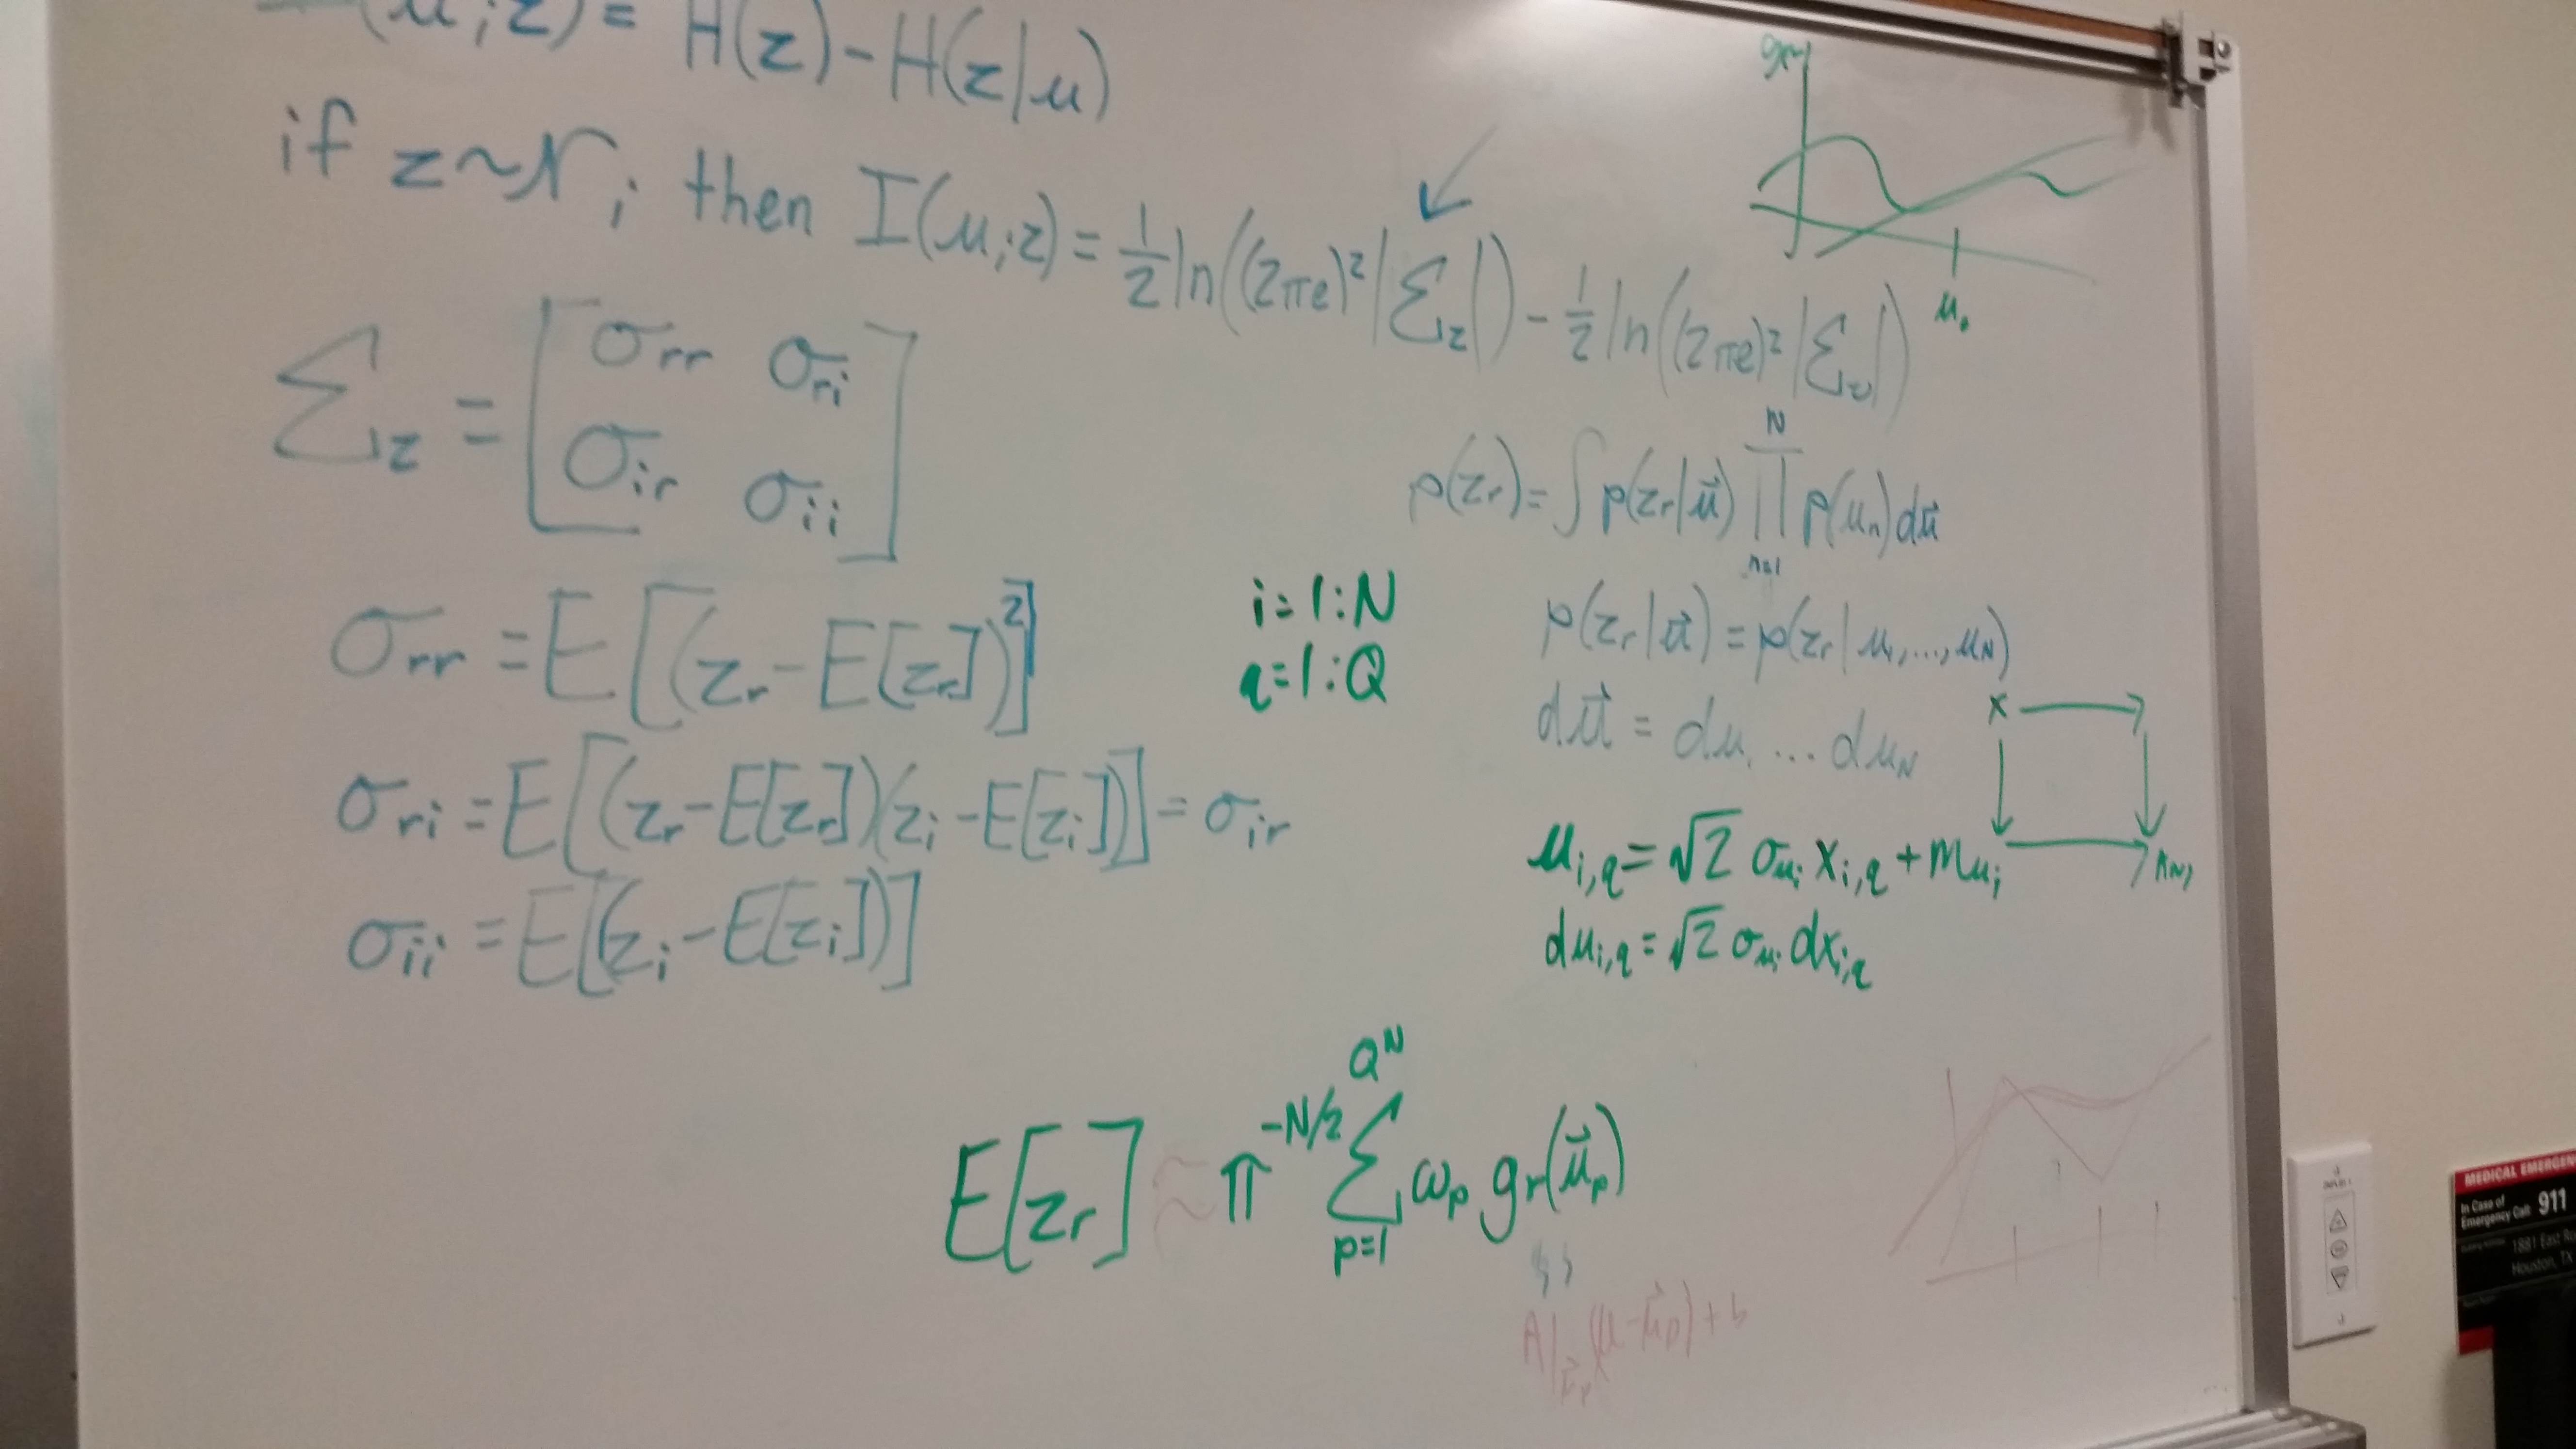
\includegraphics[width=.49\textwidth]{\picdir/20160519_115947.jpg} \\
%\end{tabular}
%\caption{ 
%\color{red}
%WIP - @dmitchell412 Need higher order entropy approximation
%}\label{fig:Pulsesequence}
%\end{figure}

\end{document}
